% ============================================================================================
% p-box cost vs. realised work (RESS). Data: validation/probability/data/pbox_cost_vs_diamonds_v2.csv
% cross-referenced against validation/probability/data/complexity_validation.csv for measured_ops.
% Fixed discretisation (steps=50), one clean timed measurement per fresh process (no same-process
% pollution), 14 networks spanning V=8..25, measured_ops=22..3112 (a 141x range).
% Paste-ready: self-contained pgfplots, no external image file needed. Matches the inline-tikz
% style already used for the adversarial crossover figure (paper_adversarial.tex).
% ============================================================================================

\begin{figure}[t]\centering
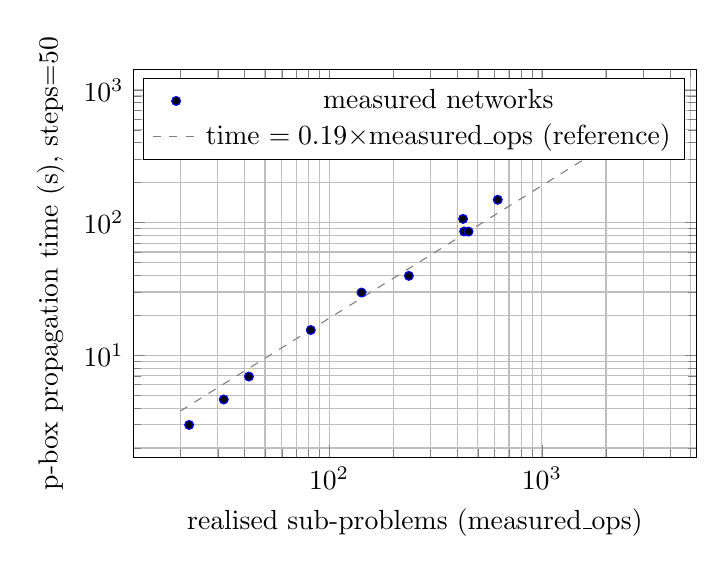
\begin{tikzpicture}
\begin{loglogaxis}[
  width=.72\linewidth, height=6.5cm,
  xlabel={realised sub-problems (measured\_ops)},
  ylabel={p-box propagation time (s), steps=50},
  grid=both,
  mark size=1.6pt,
  log basis x=10, log basis y=10,
]
\addplot+[only marks, mark=*, mark options={fill=black}] coordinates {
  (22, 2.9851)
  (32, 4.6418)
  (42, 6.9117)
  (82, 15.4937)
  (142, 29.6888)
  (237, 39.6774)
  (426, 106.6036)
  (431, 85.7466)
  (452, 85.5499)
  (620, 148.5832)
  (1564, 405.4452)
  (1747, 342.3654)
  (1961, 359.3102)
  (3112, 808.1473)
};
% Reference line: time = 0.19 * measured_ops (mid-point of the observed 0.14-0.26 s/op band)
\addplot[domain=20:3200, samples=2, dashed, gray] {0.19*x};
\legend{measured networks, time $=0.19\times$measured\_ops (reference)}
\end{loglogaxis}
\end{tikzpicture}
\caption{p-box propagation time at a fixed discretisation level (steps=50) against the realised
sub-problem count (measured\_ops) already reported for the exact/interval cost comparison
(Section~\ref{sec:complexity}), across 14 networks spanning a 141$\times$ range in measured\_ops.
Each point is a single clean measurement (one propagation per fresh process, JIT-warmed on a
throwaway network never the target -- see the methods note in Section~\ref{sec:cases}). The
near-linear relationship on log-log axes (time/measured\_ops within roughly 0.14--0.26\,s/op
throughout) shows that the same realised-work quantity governing Float64/Interval cost also
governs p-box cost, at a roughly constant price per resolved sub-problem for a given
discretisation level -- not the raw conditioning-set-width bound, which does not correlate this
cleanly (see Section~\ref{sec:numerical}).}
\label{fig:pbox_cost}
\end{figure}
